%\documentclass[12pt,letterpaper]{article}

%%%
%% Required packages:
%%
\usepackage{etex}
\usepackage{amsmath}
\usepackage{amssymb}
\usepackage{amstext}
\usepackage{amsthm}
\usepackage{fancyhdr,fancybox}
\usepackage{mathrsfs} % need for \mathscr command
\usepackage{multicol}
\usepackage[normalem]{ulem}
%\usepackage{pictex,pictexplus}
% \usepackage{pictexwd}
\usepackage{rotating}
\usepackage{url}
\usepackage{xfrac}
\usepackage{booktabs}
\usepackage{color,soul}
\usepackage{comment}

\usepackage{hyperref}
\hypersetup{
    colorlinks=true,     % false: boxed links; true: colored links
    linkcolor=blue,      % color of internal links
    citecolor=blue,      % color of links to bibliography
    filecolor=blue,      % color of file links
    urlcolor=blue        % color of external links
}


\usepackage{tikz}
\usetikzlibrary{backgrounds,calc}

%%
%% Common formatting commands
%%
\setlength{\parindent}{0in}
\setlength{\textwidth}{7in}
\setlength{\evensidemargin}{-0.25in}
\setlength{\oddsidemargin}{-0.25in}
\setlength{\parskip}{.5\baselineskip}
\setlength{\topmargin}{-0.5in}
\setlength{\textheight}{9in}

%               Problem and Part
\newcounter{problemnumber}
\newcounter{partnumber}
\newcounter{subpartnumber}
\newcommand{\Problem}{%
  \refstepcounter{problemnumber}%
  \setcounter{partnumber}{0}%
  \setcounter{subpartnumber}{0}%
  \item[\makebox{\hfil\textbf{\theproblemnumber.}\hfil}]%
  }
\newcommand{\InProblem}[2][1.6]{%
  \refstepcounter{problemnumber}%
  \setcounter{partnumber}{0}%
  \setcounter{subpartnumber}{0}%
  \textbf{\theproblemnumber.}\ \ \parbox[t]{#1in}{#2}%
}
\newcommand{\InSmallProblem}[1]{\InProblem[1.05]{#1}}
\newcommand{\NoProblem}[1]{%
  \mbox{\hfil\textbf{#1}\hfil}%
  }
\newcommand{\UnProblem}{%
  \refstepcounter{problemnumber}%
  \setcounter{partnumber}{0}%
  \setcounter{subpartnumber}{0}%
  \mbox{\hfil\textbf{\theproblemnumber.}\hfil}%
  }
\newcommand{\InFlexProblem}[1]{%
  \refstepcounter{problemnumber}%
  \setcounter{partnumber}{0}%
  \setcounter{subpartnumber}{0}%
  \textbf{\theproblemnumber.}\ \ #1%
}
%%  Part:
\newcommand{\Part}{%
  \renewcommand{\thepartnumber}{(\alph{partnumber})}%
  \refstepcounter{partnumber}
  \setcounter{subpartnumber}{0}%
  \item[(\alph{partnumber})]%
}
\newcommand{\InPart}[2][1.75]{%
  \renewcommand{\thepartnumber}{(\alph{partnumber})}%
  \refstepcounter{partnumber}%
  \setcounter{subpartnumber}{0}%
  (\alph{partnumber})\ \ \parbox[t]{#1in}{#2}%
}
\newcommand{\UnPart}{%
  \refstepcounter{partnumber}%
  \renewcommand{\thepartnumber}{(\alph{partnumber})}%
  \setcounter{subpartnumber}{0}%
  (\alph{partnumber})%
}
\newcommand{\InLargePart}[1]{\InPart[3.05]{#1}}
\newcommand{\InFullPart}[1]{\InPart[6.2]{#1}}
\newcommand{\InSmallPart}[1]{\InPart[1.05]{#1}}
%% SubPart:
\newcommand{\SubPart}{%
  \refstepcounter{subpartnumber}%
  \item[(\roman{subpartnumber})]%
  }
\newcommand{\InSubPart}[2][2.25]{%
  \stepcounter{subpartnumber}%
  (\roman{subpartnumber})\ \ \parbox[t]{#1in}{#2}%
}
\newcommand{\InSmallSubPart}[1]{\InSubPart[1.5]{#1}}
\newcommand{\InTinySubPart}[1]{%
  \stepcounter{subpartnumber}%
  (\roman{subpartnumber})\ \ \makebox{#1}%
}
\newcommand{\InMySubPart}[2][2.25]{%
  \stepcounter{subpartnumber}%
  \parbox[t]{#1in}{\makebox[0.3in][l]{(\roman{subpartnumber})}\ \ {#2}}%
}
\newcommand{\TrueFalse}{\textbf{T}\ \ \textbf{F}\ \ }
\newcommand{\TFPart}[1]{% 
  \stepcounter{partnumber}%
  \setcounter{subpartnumber}{0}%
  \item[(\alph{partnumber})] \TrueFalse\parbox[t]{5.5in}{#1}}

\newcommand{\Points}[1]{(#1 points) \ }
\newcommand{\Point}[1]{(#1 point) \ }


%% For Answers:
\newcounter{answernumber}
\newcommand{\Answer}{%
  \refstepcounter{answernumber}%
  \setcounter{partnumber}{0}%
  \setcounter{subpartnumber}{0}%
  \item[\makebox{\hfil\textbf{\theanswernumber.}\hfil}]%
  }


% Setting up the headers for the first page
%\chead{} % will default to what is typed in the file.
\fancyhead[L]{\textsc{Math 22a}}
\fancyhead[R]{\textsc{Fall 2024}}
\fancyfoot[R]{
	\vspace*{\fill}\footnotesize\textcopyright{} \emph{Harvard Math 22a}	
}
\renewcommand{\headrulewidth}{0pt}

%\fancyhead[C]{}
%	\chead{}	
%	\lhead{}
%	\rhead{}
%	\cfoot{}


% Putting copyright on the footer of each page
%\fancypagestyle{secondpage}{
%	\fancyhead[C]{TESTing again} % change this to be blank
%		%\chead{}	
%	\fancyhead[L]{bears} % change this to be blank
%	\fancyhead[R]{dogs} % change this to be blank
%	\fancyfoot[R]{ %keeps the footer the same
%		\vspace*{\fill}\footnotesize\textcopyright{} \emph{Harvard Math 22a}	
%	}
%}
%\renewcommand{\headrulewidth}{0pt}
%\pagestyle{fancy}
\pagestyle{empty}


%\lhead{}
%\rhead{}
%\rfoot{\vspace*{\fill}\footnotesize\textcopyright{} \emph{Harvard Math 22a}}
%\renewcommand{\headrulewidth}{0pt}
%\pagestyle{fancy}




%%
%% Common shortcut commands:
%%
\newcommand{\ds}{\displaystyle}
\newcommand{\sgn}{\operatorname{sgn}}
\renewcommand{\Pr}{\operatorname{P}}
\newcommand{\CPr}[3][{}]{\Pr_{\text{#1}}\left(#2\,|\,#3\right)}

\newcommand{\C}{\mathbb{C}}
\newcommand{\R}{\mathbb{R}}
\newcommand{\Z}{\mathbb{Z}}
\newcommand{\N}{\mathbb{N}}
\newcommand{\Q}{\mathbb{Q}}
\newcommand{\D}{\mathbb{D}}

\newcommand{\rref}{\operatorname{rref}}
\newcommand{\im}{\operatorname{im}}
\newcommand{\rank}{\operatorname{rank}}
\newcommand{\diag}{\operatorname{diag}}
\newcommand{\Span}{\operatorname{span}}
%\renewcommand{\vec}[1]{\mathbf{#1}}
\newcommand{\charpoly}{\mathscr{P}}
\newcommand{\nicefrac}[2]{\sfrac{#1}{#2}} % using xfrac package
\newcommand{\topology}{\mathcal{T}}
\newcommand{\Inn}{\operatorname{Inn}}

\newcommand{\blankbox}[2]{\fbox{\rule{#1}{0in}\rule{0in}{#2}}}

\newenvironment{myindentpar}[1]%
 {\begin{list}{}%
         {\setlength{\leftmargin}{#1}
          \setlength{\rightmargin}{\leftmargin}}%
         \item[]%
 }
 {\end{list}}
\newtheorem{theorem}{Theorem}
\newtheorem*{NStheorem}{Theorem}
\newtheorem{cor}[theorem]{Corollary}
\newtheorem*{claim}{Claim}
\newtheorem{defn}{Definition}

\newenvironment{amatrix}[1]{%
  \left(\begin{array}{@{}*{#1}{c}|c@{}}
}{%
  \end{array}\right)
}

%--------grstep
% For denoting a Gauss' reduction step.
% Use as: \grstep{\rho_1+\rho_3} or \grstep[2\rho_5 \\ 3\rho_6]{\rho_1+\rho_3}
\newcommand{\grstep}[2][\relax]{%
   \ensuremath{\mathrel{
       {\mathop{\longrightarrow}\limits^{#2\mathstrut}_{
                                     \begin{subarray}{l} #1 \end{subarray}}}}}}
\newcommand{\swap}{\leftrightarrow}



\section{{Mathematical Induction,  \framebox\S 10}}
\chead{\Large\textbf{Mathematical Induction,  \fbox\S 10}}

%\begin{document}
\thispagestyle{fancy}

\begin{center}
  \Ovalbox{\hspace*{.25in}\parbox{5in}{{\ \hfill\Large\rule[-.2cm]{0in}{0.9cm}\textbf{Mathematical Induction}\hfill \ }\\%
      %%
      Remember that the basic procedure of mathematical induction was
      as follows:
      \begin{enumerate}
        \item[\textbf{1.}] Prove that a statement $S_1$ is true.
        \smallskip

        \item[\textbf{2.}] Prove that, for all integers $n\ge 1$, that
          the statement $S_n$ implies the statement $S_{n+1}$: $S_n
          \implies S_{n+1}$.
        \smallskip

        \item[\textbf{3.}]  Conclude that $S_n$ is true for all
          integers $n\ge1$.
        \smallskip

      \end{enumerate}
      %%
    }\hspace*{0.25in}}
\end{center}
\bigskip

Use mathematical induction to prove the following statements:
\begin{enumerate}
  \Problem 
  Find and prove a formula for $$\sum_{j=1}^{n}{\frac{1}{j(j+1)}}.$$
  \vfill

  \Problem 
  The sum of the first $n$ squares of natural numbers is $\frac{n(n+1)(2n+1)}{6}$:
  \begin{equation*}
    \sum_{k=1}^{n} k^2 
    = 1 + 4 + 9 + \cdots + n^2
    = \frac{n(n+1)(2n+1)}{6}.
  \end{equation*}
  \vfill

  \Problem Here is an $L$-shaped tromino:
  %\begin{center}
   \raisebox{-0.1in}[0em][0em]{
\includegraphics[width=.3in]{10-induction/L-tromino}}\ .
  %\end{center}
  Show that, for all integers $n\ge1$, a $2^n\times2^n$ sheet of graph
  paper with one corner box removed can be tiled by such trominos.
  % Found at http://math.stackexchange.com/questions/145189/examples-of-mathematical-induction
  \vfill

\end{enumerate}
\newpage


\begin{center}
  \Ovalbox{\hspace*{.25in}\parbox{5in}{{\ \hfill\Large\rule[-.2cm]{0in}{0.9cm}\textbf{Strong Mathematical Induction}\hfill \ }\\%
      %%
      Remember that the basic procedure of strong mathematical induction was
      as follows:
      \begin{enumerate}
        \item[\textbf{1.}] Prove that a statement $S_1$ is true.
        \smallskip

        \item[\textbf{2.}] Prove that, for all integers $n\ge 1$, that
          the statement $S_k$ (for $k=1,2,\ldots,n$ implies the statement $S_{n+1}$: $\{S_1,S_2,\ldots,S_n\}
          \implies S_{n+1}$.
        \smallskip

        \item[\textbf{3.}]  Conclude that $S_n$ is true for all
          integers $n\ge1$.
        \smallskip

      \end{enumerate}
      %%
    }\hspace*{0.25in}}
\end{center}
\bigskip

Prove the following using strong induction:
\begin{enumerate}
  \Problem Recall that $f_k$, the Fibonacci numbers, are defined by
  $f_1 = f_2 = 1$ and $f_{n+1} = f_n+f_{n-1}$ for $n\ge 2$.  Show that
  \begin{equation*}
    f_n = \frac{\phi^n - \psi^n}{\sqrt{5}},
  \end{equation*}
  where $\phi = \frac{1+\sqrt{5}}{2}$ is the \emph{golden ratio}\ and
  $\psi = \frac{1-\sqrt{5}}{2} = -1/\phi$.
  \vfill
\end{enumerate}

%\end{document}
\begin{comment}

\newpage
\chead{\Large\textbf{Mathematical Induction -- Answers / Solutions}}%
\lhead{}
\rhead{}
\thispagestyle{fancy}

\begin{enumerate}
  \Answer Find and prove a formula for $$\sum_{j=1}^{n}{\frac{1}{j(j+1)}}.$$
  \begin{proof}
  	We'll begin by finding a formula. Using some basic calculations, we see that the first sum is $\frac{1}{2}$ and the next is $\frac{1}{2} + \frac{1}{6} = \frac{2}{3}$, and the one after is $\frac{2}{3} + \frac{1}{12} = \frac{3}{4}$. So a natural guess would be that the sum of the first $n$ such fractions is $\frac{n}{n+1}$. 
  	
  	\textbf{Base Case:} (We covered this above but I'll write it out here for the proof) For $n=1$, we have that the sum is: $\sum_{j=1}^1 \frac{1}{j(j+1)} = \frac{1}{(1)(2)} = \frac{1}{2}$, which agrees with our formula.
  	
  	\textbf{Inductive Hypothesis:} Suppose that this formula works for some $n$, so $\sum_{j=1}^{n}{\frac{1}{j(j+1)}} = \frac{n}{n+1}$ for some specific $n$.
  	
  	\textbf{Inductive Step:} Now we need to show that the formula works for $n+1$, assuming that it works for $n$. So we want to show that the sum $$\sum_{j=1}^{n+1} \frac{1}{j(j+1)} = \frac{n+1}{n+2}.$$
  	$$\sum_{j=1}^{n+1} \frac{1}{j(j+1)} = \sum_{j=1}^n \frac{1}{j(j+1)} + \frac{1}{(n+1)(n+2)} = \frac{n}{n+1} + \frac{1}{(n+1)(n+2)} $$ $$= \frac{n(n+2) + 1}{(n+1)(n+2)} = \frac{n^2 + 2n + 1}{(n+1)(n+2)} = \frac{(n+1)^2}{(n+1)(n+2)} = \frac{n+1}{n+2} $$
  	And we're done!
  	
  \end{proof}

  \Answer The sum of the first $n$ squares of natural numbers is $\frac{n(n+1)(2n+1)}{6}$:
  \begin{equation*}
    \sum_{k=1}^{n} k^2 
    = 1 + 4 + 9 + \cdots + n^2
    = \frac{n(n+1)(2n+1)}{6}.
  \end{equation*}
  
    \begin{proof}
  	We want to proceed by induction!
  	
  	\textbf{Base Case:} For $n=1$, we have that the sum is: $\sum_{k=1}^1 k^2 = 1 = \frac{1(1+1)(2(1)+1)}{6}$, which agrees with our formula.
  	
  	\textbf{Inductive Hypothesis:} Suppose that this formula works for some $n$, so $\sum_{k=1}^n = \frac{n(n+1)(2n+1)}{6}$.
  	
  	\textbf{Inductive Step:} Now we need to show that the formula works for $n+1$, assuming that it works for $n$. So we want to show that the sum $$\sum_{k=1}^{n+1} k^2  = \frac{(n+1)(n+2)(2(n+1)+1)}{6} = \frac{(n+1)(n+2)(2n+3)}{6}.$$
  
  Here we have
  	$$\sum_{k=1}^{n+1} k^2 = \sum_{k=1}^n k^2 + (n+1)^2 =  \frac{n(n+1)(2n+1)}{6} + n^2 + 2n + 1 =  \frac{(n^2+n)(2n+1)}{6} + n^2 + 2n + 1 $$ $$= \frac{2n^3 + 3n^2 + n}{6} + n^2 + 2n + 1 = \frac{2n^3 + 9n^2 + 13n + 6}{6} = \frac{(n+1)(n+2)(2n+3)}{6} $$
  	And we're done!
  	
  \end{proof}

  \Answer 
  
  \begin{proof}
  We prove the result by induction.
  
  {\bf Base Case:} For $n=1$, we have a 2 by 2 square with one corner removed. This is exactly our tromino, and hence the base case holds.
  
  {\bf Inductive Hypothesis:} Suppose a $2^n \times 2^n$ sheet with one corner removed can be covered.
  
  {\bf Inductive Step:}  Consider a $2^{n+1}$ by $2^{n+1}$ sheet of graph paper with one corner removed. Dividing the sheet in half, we get four $2^n \times 2^n$ sheets, one of which has a corner removed. We can apply the induction hypothesis to the one with the corner removed to conclude that one can be removed by the trominos. Placing one tromino at the middle of the sheet can cover one corner from each of the remaining sheets. Now we apply the induction hypothesis to the three remaining sheets yields a covering of the entire sheet. Thus by induction, we can cover the entire sheet. Here is a picture illustrating the placement.
  
  \begin{center}
  \begin{tikzpicture}
  \draw[step=1.0,black,thin] (0,0) grid (8,8);
  \draw[line width=1mm] (4,0) -- (4,8);
  \draw[line width=1mm] (0,4) -- (8,4);
  \fill[white] (7.01,7.01)--(7.01,8.1)--(8.1,8.1)--(8.1,7.01)--(7.01,7.01);
  \fill[yellow] (3,3) -- (5,3) -- (5,4) -- (4,4) -- (4, 5) --(3,5)--(3,3);
  \end{tikzpicture}
  \end{center}
  
  \end{proof}

  \Answer Recall that $f_k$, the Fibonacci numbers, are defined by
  $f_1 = f_2 = 1$ and $f_{n+1} = f_n+f_{n-1}$ for $n\ge 2$.  Show that
  \begin{equation*}
    f_n = \frac{\phi^n - \psi^n}{\sqrt{5}},
  \end{equation*}
  where $\phi = \frac{1+\sqrt{5}}{2}$ is the \emph{golden ratio}\ and
  $\psi = \frac{1-\sqrt{5}}{2} = -1/\phi$.

  \begin{proof}
  	\textbf{Base Case:} Note that we want to prove an induction statement that depends on two cases. So we need to show that this works for $n=1$ and $2$:
  	$$f_1 = 1 = \frac{\sqrt{5}}{\sqrt{5}} =  \frac{\phi - \psi}{\sqrt{5}}$$
  	$$f_2 = 1 = \frac{4 \sqrt{5}}{4\sqrt{5}} =  \frac{ 1 + 2\sqrt{5} + 5 - (1 - 2\sqrt{5} + 5)}{4\sqrt{5}} = \frac{\phi^2 - \psi^2}{\sqrt{5}}$$
  	
  	\textbf{Inductive Hypothesis:} Suppose that this formula works for all $k$ with $1 \leq k \leq n$.
  	
  	\textbf{Inductive Step:} Now we need to show that the formula works for $n+1$, assuming that it works for all $1 \leq k \leq n$. Note that $\phi^2 = 1 + \phi$, and $\psi^2 = 1 + \psi$. We have that $f_{n+1} = f_n + f_{n-1}$ by the defn. of Fibonacci numbers, and so we can use our induction hypothesis here to substitute. Note that we needed strong induction because our usual induction hypothesis would \textbf{only} gives us $f_n$, not $f_n$ and $f_{n-1}$. Substituting in, we get:
  	$$f_{n+1} = \frac{\phi^n - \psi^n}{\sqrt{5}} + \frac{\phi^{n-1} - \psi^{n-1}}{\sqrt{5}} = \frac{\phi^{n-1} (\phi + 1) - \psi^{n-1} (\psi + 1)}{\sqrt{5}}$$
  	We can now substitute using $\psi^2 = 1 + \psi$ to get:
  	$$\frac{\phi^{n-1} (\phi^2) - \psi^{n-1} (\psi^2)}{\sqrt{5}} =  \frac{\phi^{n+1} - \psi^{n+1}}{\sqrt{5}}$$
  	which proves our formula.
  \end{proof}

\end{enumerate}

\end{comment}
%\end{document}


%%% Local Variables: 
%%% mode: latex
%%% TeX-master: t
%%% End: 
